\documentclass[__main__.tex]{subfiles}

\begin{document}

\qtitle{О}{11}
Между точечным источником света $S$ и точкой наблюдения $P$ расположили круглую диафрагму, центр которой совпадает с осью $SP$. Покажите, что расстояние от оси, соединяющей точечный источник и точку наблюдения, до границы $n$-й зоны Френеля даётся соотношением $r_n=\sqrt{n\lambda\frac{ab}{a+b}}$, где $\lambda$ -- длина волны, $a$ -- расстояние от источника до диафрагмы, $b$ -- расстояние от диафрагмы до точки наблюдения.\\ 

\begin{wrapfigure}{R}{.4\linewidth}
    \centering
    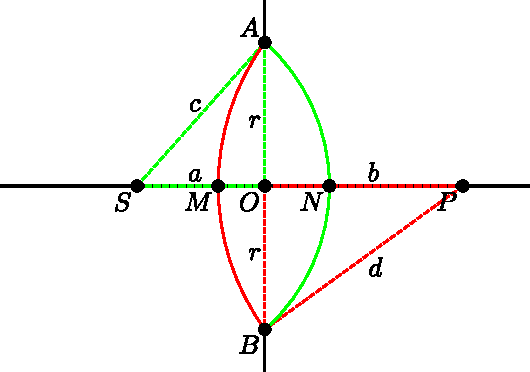
\includegraphics[width=1\linewidth]{О-11_1}
    \caption{}
    \llabel{o11:scheme}
\end{wrapfigure}

Рассмотрим диафрагму $AB$ радиуса $r$. Тогда получим схему задачи (см. Рис. \lref{o11:scheme}), где $a=SO$ -- расстояние от источника до диафрагмы, $b=PO$ -- расстояние от точки наблюдения до диафрагмы, $r=AO=OB$ -- радиус диафрагмы. Радиус диафрагмы $r$ положим намного меньшим, чем расстояния от диафрагмы до источника и точки наблюдения:
\begin{gather}
r\ll{a},
\qquad
r\ll{b}
\llabel{o11:mans}
\end{gather}
Построим волновую поверхность $ANB$: сферу радиуса $c=\sqrt{a^2+r^2}$, также построим сферу радиуса $d=\sqrt{b^2+r^2}$ с центром в точке $P$. Тогда радиус $m$-ой зоны Френеля имеет вид $R_{n}=R_{0}+\frac{n\lambda}{2}$, где $R_{0}=NP$: положим, что диафрагма открывает ровно $n$ зон Френеля, получим:
\begin{flalign*}
&
\begin{cases}
R_{n}=PB=d\\
R_{0}=NP=a+b-c\\
\end{cases}
\Longleftrightarrow
R_{n}-R_{0}=\frac{n\lambda}{2}
\Longleftrightarrow\\
\Longleftrightarrow&
c+d-a-b=\frac{n\lambda}{2}
\Longleftrightarrow
\sqrt{a^2+r^2}-a+\sqrt{b^2+r^2}-b=\frac{n\lambda}{2}
\Longleftrightarrow\\
\Longleftrightarrow&
a\left[\sqrt{1+\frac{r^2}{a^2}}-1\right]
+
b\left[\sqrt{1+\frac{r^2}{b^2}}-1\right]
=
\frac{n\lambda}{2},
\end{flalign*}
теперь, согласно (\lref{o11:mans}), можем воспользоваться эквивалентностью $(1+x)^n-1\sim{nx}$, чтобы получить \emph{приближенное} решение:
\begin{flalign}
&
r^2\left(\frac{1}{2a}+\frac{1}{2b}\right)=\frac{n\lambda}{2}
\Longleftrightarrow\\
\Longleftrightarrow&
r^2=\frac{n\lambda}{1/a+1/b}
\Longleftrightarrow\\
\Longleftrightarrow&
r_{n}=\sqrt{n\lambda\frac{ab}{a+b}}
\end{flalign}


\end{document}